\documentclass{article}
\usepackage{listings}
\usepackage{graphicx}
\usepackage{hyperref}
\usepackage{xcolor}
\usepackage{amsmath}

\definecolor{codegreen}{rgb}{0,0.6,0}
\definecolor{codegray}{rgb}{0.5,0.5,0.5}
\definecolor{codepurple}{rgb}{0.58,0,0.82}
\definecolor{backcolour}{rgb}{0.95,0.95,0.92}

\hypersetup{
    colorlinks=true, % Set to true to enable colored links
    linkcolor=black, % Color of internal links
    filecolor=magenta, % Color of file links
    urlcolor=black, % Color of external url links
    citecolor=black % Color of citations
}

\lstdefinestyle{mystyle}{
    backgroundcolor=\color{backcolour},   
    commentstyle=\color{codegreen},
    keywordstyle=\color{magenta},
    numberstyle=\tiny\color{codegray},
    stringstyle=\color{codepurple},
    basicstyle=\ttfamily\footnotesize,
    breakatwhitespace=false,         
    breaklines=true,                 
    captionpos=b,                    
    keepspaces=true,                 
    numbers=left,                    
    numbersep=5pt,                  
    showspaces=false,                
    showstringspaces=false,
    showtabs=false,                  
    tabsize=2
}

\lstset{style=mystyle}

\title{ChildSynth: Leveraging Synthetic Imagery for Automated Height Measurement in Malnutrition Prediction}
\author{David Berthiaume, Catherine Gai, Chau Nguyen, \\Yuan Tang, Emilia Mazzolenis}

\begin{document}

\maketitle
\tableofcontents


\section{Introduction}

Predicting childhood malnutrition is a critical task in the field of public health. Malnutrition among children is still a significant public health problem in many developing countries. It is a primary cause of morbidity and mortality in children. Malnutrition is a condition that results from eating a diet in which one or more nutrients are insufficient, such that the diet causes health problems.

This paper proposes a novel approach to predict malnutrition in children using synthetic imagery. 
We leverage the power of synthetic data to help evaluate and train several deep-learning models to predict heights in children to support the prediction of malnutrition. 

Obtaining data for training deep learning models is a challenging task. The data must be labeled and annotated, which can be time-consuming and expensive. Obtaining images of children to train a model to predict malnutrition is even more challenging. These images and height measurements must be taken in a controlled environment with trained personnel to ensure high accuracy. Furthermore, this data is highly sensitive since it involves images of children.

To combat these challenges, a synthetic data generator, ChildSynth, was developed to create images of children with pixel-perfect height measurements. This synthetic data generator can create an unlimited number of images of children with varying characteristics and pixel-perfect heights. The generated synthetic data can be used to evaluate and pre-train deep learning models to predict children's height. 

\section{ChildSynth}

ChildSynth is a command-line program that uses procedural modeling and raytracing powered by Pov-RAY~\cite{povray} to generate color images, depth maps, segmentation maps, keypoints, precise height measurements, and auxiliary information for synthetic children lying on a mat as viewed from different camera angles. The following example command generates RGB images, depth maps, segmentation maps, and auxiliary text files with height measurements and other characteristics for $5$ different camera angles for a total of $15$ images. 

\begin{lstlisting}[language=bash]
python render_children.py --resy 512 --resx 512 --num_children 1     --output_dir ./output 
\end{lstlisting}

Figure \ref{fig:child_0} shows an example of a synthetic child generated by the above command.

\begin{figure}[]
    \centering
    \includegraphics[width=\textwidth]{plots/child_0.png}
    \caption{Example of a synthetic child generated by ChildSynth. The upper row consists of color images, the middle row consists of depth maps, and the bottom row consists of binary segmentation maps indicating whether each pixel is part of a child or part of the background.}
    \label{fig:child_0}
\end{figure}

The goal of ChildSynth is not to generate photorealistic images but to parametrically model children with infinite variations and with pixel-perfect measurements. Every element, the length, style, density, and color of hair, the facial characteristics, the skin and mat textures, even the size of each toe, is modeled parametrically and can be individually specified or sampled from various random distributions. Elements of the scene, including camera position, lighting, and image quality, are also parametrically modeled. One can specify over $100$ different parameters to control how the children and scenes are rendered. 

Photorealistic images are not always necessary for achieving excellent results in training computer vision models. Depending on the specific application and tasks, computer vision systems can be effectively trained using synthetic or stylized imagery that does not mimic the full complexity of real-world visuals but instead retains essential structural and contextual elements needed for the model to learn and perform accurately. For example, non-photorealistic rendering was successfully used to train models for autonomous driving in complex urban environments under many weather conditions, where logistical challenges prevent training and testing such systems in the physical world~\cite{dosovitskiy2017carla}. Non-photorealistic rendering was also successfully used by OpenAI for reinforcement learning applications in robotics~\cite{openai2018dexterous}. Furthermore, using realistic static meshes or generative AI would greatly reduce this flexibility and make it difficult to generate the vast number of images with precise and exhaustive measurements needed to train a deep-learning model. 

This fully parametric modeling provides two primary benefits.

\begin{itemize}

    \item \textbf{Explainability:} By providing precise measurements for over $100$ different feature of the generated image, this data provides a rich environment for explainability. For example, by analyzing the metadata attached to each image, one may find that a particular model is performing poorly on synthetic images where a child has long hair, the clothing is particularly wrinkled, or their legs are in a certain position relative to the body.  
    
    \item \textbf{Generalizability:} Height prediction is just one of the many tasks that this synthetic dataset generator could be used for. Any parameter such as body widith, leg length, leg position, or even key point locations (explained below) could be used a prediction task. Combining multiple prediction tasks together could help with model generalizability.

\end{itemize}

\section{Approach}
\subsection{Rendering}

ChildSynth renders each parametrically modeled scene using ray tracing. The geometries in the scene are composed of spheres, cylinders, cubes, rounded cubes, triangles, planes, and BLOBs (Binary Large OBjects), explained below. 

Each child is rendered from multiple view angles to provide a variety of perspectives. The camera is placed at different positions above the child to capture the child's body from multiple positions. By default, $5$ different camera angles are used to render each child, from $30$ to $150$ degrees, in increments of $30$ degrees, with $90$ degrees being directly above the child, and $30$ and $150$ degrees being to the left and right of the child respectively. These multiple views allow one to predict the child's height with multi-view computer vision approaches.




ChildSynth renders a depth image corresponding to each color image by storing the distance from the camera to the first solid ray intersection in the scene. This depth image and the color imagery are precisely co-registered.

Finally, ChildSynth renders a segmentation map for each child. The segmentation map is a binary image where each pixel is equal to $1$ if it is part of the child and $0$ if it is part of the background. Along with the color and depth images, the segmentation map is helpful for training deep-learning models to predict the child's height.


\subsection{Modeling}

\subsubsection{Randomness}

ChildSynth can render millions of synthetic children, with no two being identical.  It accomplishes this by sampling over $100$ parameters from various probability distributions. For example, ChildSynth may place an optional spotlight around the child as a light source. The position of this spotlight is sampled from several normal distributions, with the light being most likely placed near the child. The color of this light source is sampled from three uniform distributions, one for each of the red, green, and blue intensities. 

Several distributions are available in ChildSynth; all parameters can be optionally specified in the command line and support every probability distribution. Every parameter has a default distribution that is used when no distribution is explicitly provided.

\subsubsection{Probability Distributions}

This section provides a summary of the available probability distributions and their arguments. The following distributions are available in ChildSynth:

\begin{itemize}

    \item {\textbf{Constant}: The simplest distribution defines a single constant value that is selected with probability $1$.}
    
    Example usage:
    \begin{lstlisting}[language=bash]
python render_children.py --smile_factor constant:0.7 \end{lstlisting}
    
    \item \textbf{Bernoulli}: The Bernoulli distribution defines a probability $p$ that a binary random variable is equal to $1$. This can be used to turn on or off features such as an individual light source, or the rendering of hari. 
    
    Example usage:
    \begin{lstlisting}[language=bash]
python render_children.py --spotlight_1 bern:0.3\end{lstlisting}
   
    \item \textbf{Uniform}: The uniform distribution is defined by two parameters, $a$ and $b$, which are the minimum and maximum values of the distribution. 
    
    Example usage:
    \begin{lstlisting}[language=bash]
python render_children.py --hair_color_red unif:0.1,0.6\end{lstlisting}
    
    \item \textbf{Normal}: The normal distribution is defined by two parameters, $\mu$ and $\sigma$, which are the mean and standard deviation of the distribution.
    
    Example usage:
    \begin{lstlisting}[language=bash]
python render_children.py --head_size normal:0.8,0.2\end{lstlisting}
    
    \item \textbf{Binomial}: The binomial distribution is used to sample an integer obtained from $n$ independent Bernoulli samples with probability $p$. This returns the number of successes in these independent trials. To use this distribution, one specifies the number of trials $n$, and then the probability of success for each independent trial $p$. 
    
    Example usage:
    \begin{lstlisting}[language=bash]
python rener_children.py  --clothes_wrinkles binom:100,0.5\end{lstlisting}

    \item \textbf{Choice}: The choice option provides a way of selecting an integer from $0$ to a maximum value (exclusive) with uniform probability. This allows one to select from a list of options. For example, the texture for the mat is one of $100$ possible textures, and the choice distribution is used to select one of these textures.  
    
    Example usage:
    \begin{lstlisting}[language=bash]
python rener_children.py --mat_texture choice:100\end{lstlisting}
        
        
\end{itemize}

\subsection{Colors}
ChildSynth supports the specification of colors using the RGB color space where each of the red, green, and blue values lie in the range $[0,1]$. Each channel is specified separately using subparameters separated by an underscore to allow maximum flexibility. The following example specifies the color of hair with a red intensity of $1$, a blue intensity of $0.25$, and a green intensity sampled from a normal distribution with a mean of $0.2$ and a standard deviation of $0.1$. See figure \ref{fig:red_hair}.


\begin{lstlisting}[language=bash]
python render_children.py --hair_color_red 1 --hair_color_blue 0.25 --hair_color_green normal:0.5,0.1\end{lstlisting}

\begin{figure}[htbp]
    \centering
    \includegraphics[height=3.7cm]{plots/child_000000_rgb_060.png}
    \includegraphics[height=3.7cm]{plots/child_000000_rgb_090.png}
    \includegraphics[height=3.7cm]{plots/child_000000_rgb_120.png}
    \caption{Hair color is specified with red, green, and blue intensities. The red and blue intensities are set to $1$ and $0.25$, respectively, while the green intensity is sampled from a normal distribution with a mean of $0.2$ and a standard deviation of $0.1$.}
    \label{fig:red_hair}
\end{figure}

\subsection{Vectors}

ChildSynth similarly supports specifying vectors with subcomponents. For example, one can rotate the child along the x,y, and z axes. To rotate the child $180$ degrees along the z-axis (the z-axis points into the scene) and perform a random translation along the x-axis, one can use the following syntax. See figure \ref{fig:rotation}.


\begin{lstlisting}[language=bash]
python rener_children.py  --child_rotate_z constant:3.1415 --child_shift_x unif:-1.0,1.0\end{lstlisting}

\begin{figure}[htbp]
    \centering
    \includegraphics[height=3.7cm]{plots/child_000000_rgb_030a.png}
    \includegraphics[height=3.7cm]{plots/child_000000_rgb_090a.png}
    \includegraphics[height=3.7cm]{plots/child_000000_rgb_150a.png}
    \caption{Rotating the child and providing a random shift in the x-direction}
    \label{fig:rotation}
\end{figure}

By combining shifting with rotation, we obtain an image of a child standing on the mat.

\begin{figure}[htbp]
    \centering
    \includegraphics[height=3.7cm]{plots/child_000000_rgb_030d.png}
    \includegraphics[height=3.7cm]{plots/child_000000_rgb_090d.png}
    \includegraphics[height=3.7cm]{plots/child_000000_rgb_150d.png}
    \caption{Using a combination of shift and rotation allows us to obtain an image of a child standing on the mat instead of lying down.}
    \label{fig:standing}
\end{figure}

\begin{lstlisting}[language=bash]
render_children.py --child_rotate_x constant:-90 --child_shift_z constant:0.9 --child_shift_y constant:0.4 --camera_distance constant:11\end{lstlisting}

\section{Geometry}

\subsection{BLOBs (Binary Large OBjects)}

Most of the geometry of the synthetic children is composed of BLOBs. BLOBs are a powerful tool for creating smooth shapes parametrically with ray tracing.

BLOBs are created from one or more subcomponents, each typically defined by a field of influence. These fields influence the density of the medium at their respective locations. When combined, they create a smooth surface based on a density threshold, meaning the surface of the BLOB is defined wherever the combined density of all influence spheres exceeds this threshold.

For example, consider a simple BLOB composed of two spheres. Sphere $1$ has center $c_1 = (0, 0, 0)$, radius $r_1 = 1$, and strength $s_1 = 1.5$. Sphere $2$ has  center $c_2 = (1, 0, 0)$, radius $r_2 = 1$, and strength $s_2 = 1.5$. 

We define a threshold $t_r$ that determines how spread out and smooth the shape is. A lower threshold means a larger, more spread-out blob as the surface includes points with lower summed field strengths. A higher threshold creates a tighter, smaller blob because only points with higher field strengths are included.

The influence functions for each sphere are given by
$$
f_1(p) = 1.5 \left( 1 - \frac{\| p - (0, 0, 0) \|^2}{1^2} \right)^2 
$$
$$
f_2(p) = 1.5 \left( 1 - \frac{\| p - (1, 0, 0) \|^2}{1^2} \right)^2 
.$$

The total strength at any point $p$ is
$$
S(p) = f_1(p) + f_2(p).
$$
The points, $p$, inside the BLOB are all $p$ such that $S(p) \geq t_r$.

Blobs can consist of spheres and cylinders, and the strength and shape of each sphere and cylinder can be individually controlled to create a wide variety of shapes from the resulting field.  These composite objects are beneficial for creating smooth shapes with fine-grained control over the individual features of the shape. Much of the complexity of the child's body is modeled using BLOBs, especially for the feet and hands (see figure \ref{fig:hand_foot}). 

\begin{figure}[htbp]
    \centering
    \includegraphics[height=2.6cm]{plots/hand.png}
    \includegraphics[height=2.6cm]{plots/back.png}
    \includegraphics[height=2.6cm]{plots/foot.png}
    \caption{Hands and feet are rendered using BLOBs that consist of a complex arrangement of parametric spheres and cylinders. The strength and shape of each sphere and cylinder can be individually controlled to create a wide variety of shapes from the resulting field.}
    \label{fig:hand_foot}
\end{figure}

\subsection{Procedural Character Generation}
ChildSynth uses a hierarchical modeling approach to create the child's body, with a central skeleton and parametric definitions for parent-child relationships. These parent-child relationships change dynamically as the different body parts are generated based on the samples from the random distributions. For example, the allowed upper arm rotations change based on the position and rotation of the main body to ensure that the arms are positioned realistically and that there is no clipping with the mat below.

ChildSynth defines every body part and object in the scene by a set of parameters and a set of rules to assemble those parameters into a geometry. For example, the upper leg is defined as a blob that is composed of a main cylinder and several spheres. These sub-components are generated based on the upper leg length, upper leg circumference, and the upper leg starting and ending positions. 

\subsection{The Mat}

The primary goal of ChildSynth is to provide sufficient challenge for the neural network when predicting a child's height. It is important therefore not to have any static clues that the model can heavily rely on to directly predict the child's height. For example, if a static mesh was used for the mat with a fixed size, the model could pick up on the size of the mat and use it to predict the relative height of the child. To prevent this, the mat is dynamically generated. Furthermore, these mats are likely not to be perfectly flat. 

The mat is generated by creating a heightfield from Simplex noise~\cite{perlin2001improving} and then triangulating the resulting mesh to simulate wrinkles. Figure \ref{fig:mat} shows an example mat created from a triangulated heightfield. Like all geometries in the scene, the characteristics of the generated wrinkles in the mat are controlled by a set of parameters that are sampled from various probability distributions.

\begin{figure}[]
    \centering
    \includegraphics[width=.4\textwidth]{plots/mesh.png}
    \caption{The geometry of the mat is created by triangulating a heightfield created using simplex noise. This simulates wrinkles in the mat and prevents the neural network from relying too heavily on the size of the mat to estimate the child's height.}
    \label{fig:mat}
\end{figure}

\subsection{Hair}

Hair is rendered using a combination of cylinders. Hair density, color, width variation, and length are all controllable random parameters. Hair is an important feature since it can make it more difficult to predict height since it hides the precise location of the top of the head.

\section{Materials}
\subsection{Static Textures}
The material for the mat that the child is lying on is sampled from $100$ static public domain textures which are available from \url{OpenGameArt.org}~\cite{100_seamless_textures}. These textures help provide a significant amount of variety in the background of the images, which helps prevent the neural network from expecting a specific type of background. The textures are sampled using the choice distribution by default, which allows one to select one of the $100$ textures with uniform probability. Like all parameters, other sampling options are available. For example, if one wanted to create $10,000$ images of different children lying on the same mat, one could use the constant option when specifying the mat texture.

\subsection{Dynamic Textures}

Most of the textures in the scene are generated dynamically. 

\subsubsection{Clothing Textures}

Clothing typically has wrinkles and imperfections that are difficult to model procedurally. To create realistic clothing textures, ChildSynth uses a combination of procedural modeling, simplex noise, and normal maps. Having a perfectly smooth texture for the clothing would be unrealistic and cause the neural network to expect something that would not be present in real-world images. To simulate wrinkles in the clothing, a normal map is procedurally generated using simplex noise and then applied to the geometry. 

\subsubsection{Face}

A dynamic texture is created for the face of every child to provide basic facial features. This texture is rendered from scratch using pycairo~\cite{pycairo}. The face texture is created by drawing a series of shapes, such as circles, rectangles, and lines, to create a face with eyes, a nose, and a mouth. The color of the face by default is sampled from a normal distribution to provide a wide variety of skin tones. Figure \ref{fig:faces} shows four example face textures.


\begin{figure}[htbp]
    \centering
    \includegraphics[height=2.0cm]{plots/face.png}
    \includegraphics[height=2.0cm]{plots/face4.png}
    \includegraphics[height=2.0cm]{plots/face2.png}
    \includegraphics[height=2.0cm]{plots/face3.png}
    \caption{Example face textures rendered dynamically using pycairo. The color of the face is sampled from a normal distribution to provide a wide variety of skin tones and is chosen to closely match the skin color of the rest of the child's body.}
    \label{fig:faces}
\end{figure}

\section{Lighting}
By default, ChildSynth provides $4$ light sources in each scene, two point lights, and two spot lights. The intensity of these lights is sampled from a uniform distribution to provide soft lighting for the scene with lights being provided from multiple directions. Each of these lights can by controlled by tuning the intensity and their positions.  Figure \ref{fig:lighting} shows an example of a single child rendered with various light configurations.

\begin{figure}[htbp]
    \centering
    \includegraphics[height=2.0cm]{plots/light0.png}
    \includegraphics[height=2.0cm]{plots/light2.png}
    \includegraphics[height=2.0cm]{plots/light3.png}
    \includegraphics[height=2.0cm]{plots/light4.png}
    \includegraphics[height=2.0cm]{plots/light5.png}
    \caption{A single child rendered with various light configurations. The intensity and position of each light source can be controlled to provide a wide variety of lighting conditions.}
    \label{fig:lighting}
\end{figure}

\section{Image Quality}

ChildSynth provides the ability to add noise to the rendered images to simulate real-world image noise. This noise is sampled from a Gaussian distribution with a mean of $0$ and a standard deviation that can be controlled by the user. The noise is added to the color image and the depth map. Figure \ref{fig:noise} shows an example of a child rendered with varying levels of image noise. An additional noise type is provided to exclude small patches of the image and depth maps to simulate the effect of dropout in the neural network.

\begin{figure}[htbp]
    \centering
    \includegraphics[height=2.0cm]{plots/noise0.png}
    \includegraphics[height=2.0cm]{plots/noise1.png}
    \includegraphics[height=2.0cm]{plots/noise2.png}
    \includegraphics[height=2.0cm]{plots/noise4.png}

    \caption{A single child rendered with various noise levels. The noise is sampled from a Gaussian distribution with a mean of $0$ and a standard deviation that can be controlled by the user. Optionally, box noise can be applied to the image.}
    \label{fig:noise}
\end{figure}

\section{Metadata}

ChildSynth provides a metadata file for each rendered image that contains the height of the child along with dozens of other parameters that could be used for prediction tasks, including all of the random parameters used in the scene, the camera position, the lighting conditions, the image quality, and all keypoints, both the 3D coordinates and the 2D pixel coordinates. This metadata file is saved in text format. The following is an example of a portion of a metadata file or a single render. One could use this information to train a neural network to predict hair color or the distance of the camera for example.

\begin{lstlisting}[caption={Example metadata file}]
child height (cm): 67.158385699556 
seed: 8849
head_size: 0.6278060285782697
skin_color: [1.         0.82084211 0.6872982 ]
shorts_color: [0.25174322 0.75774645 0.9093296 ]
mat_texture: 134
camera_distance: 6.356927988745477
left_arm_angle_z: 4.368737569654856
left_leg_angle_xy: 3.1419316489141185
right_leg_angle_xy: 0.5898018863921284
right_leg_angle_z: 7.382191122717593
...
image_noise_level: 50.0
child_shift_x: 0.036170449604526644
child_shift_y: -0.01152100235935788
child_shift_z: -0.01516996620636548
head_height: 2.7301132563995303
child_height: 3.3579192849778003
...
keypoint_head_top_3d: (0, 3.3579192849778, 0)
keypoint_head_top_2d: [0.5        0.26903642]
keypoint_right_hand_3d: [1.49995483 1.98835873 0.        ]
keypoint_right_hand_2d: [0.65287157 0.41658571]
keypoint_right_foot_3d: (0.32340664142017084, -0.15972602703812186, 0.0)
keypoint_right_foot_2d: [0.53556515 0.68685025]
keypoint_neck_3d: (0, 2.1023072278212607, -0.31)
keypoint_neck_2d: [0.49880674 0.39188964]
keypoint_hip_3d: (0.0, 1.0, -0.31)
keypoint_hip_2d: [0.49875394 0.52880559]
\end{lstlisting}
\section{Keypoints}
Many computer vision tasks require keypoint detection such as object tracking, pose estimation, and facial recognition. ChildSynth provides the ability to generate pixel-perfect keypoint annotations for each child. The keypoints are generated based on the dynamic geometry of the children and are then projected onto image space and saved to the metadata file associated with each view. Figure \ref{fig:keypoints} shows an example of keypoint annotations for a child lying on a mat. Keypoints are provided for the top of the head, the neck, the hip, and the feet and hands. 

\begin{figure}[]
    \centering
    \includegraphics[width=\textwidth]{plots/kpoint.png}
    \caption{Pixel-perfect keypoint annotations for a child lying on a mat. Keypoints are provided for the top of the head, the neck, the hip (rendered in red), and the feet (rendered in yellow) and hands (rendered in green).}
    \label{fig:keypoints}
\end{figure}

\section{Conclusion}
ChildSynth is a powerful tool for generating synthetic imagery of children with pixel-perfect measurements for use in evaluating and training computer vision models. It is fully customizable and can generate an unlimited number of images with varying characteristics. Figure \ref{fig:variety} shows $15$ different synthetic children rendered with default parameters.

\begin{figure}[]
    \centering
    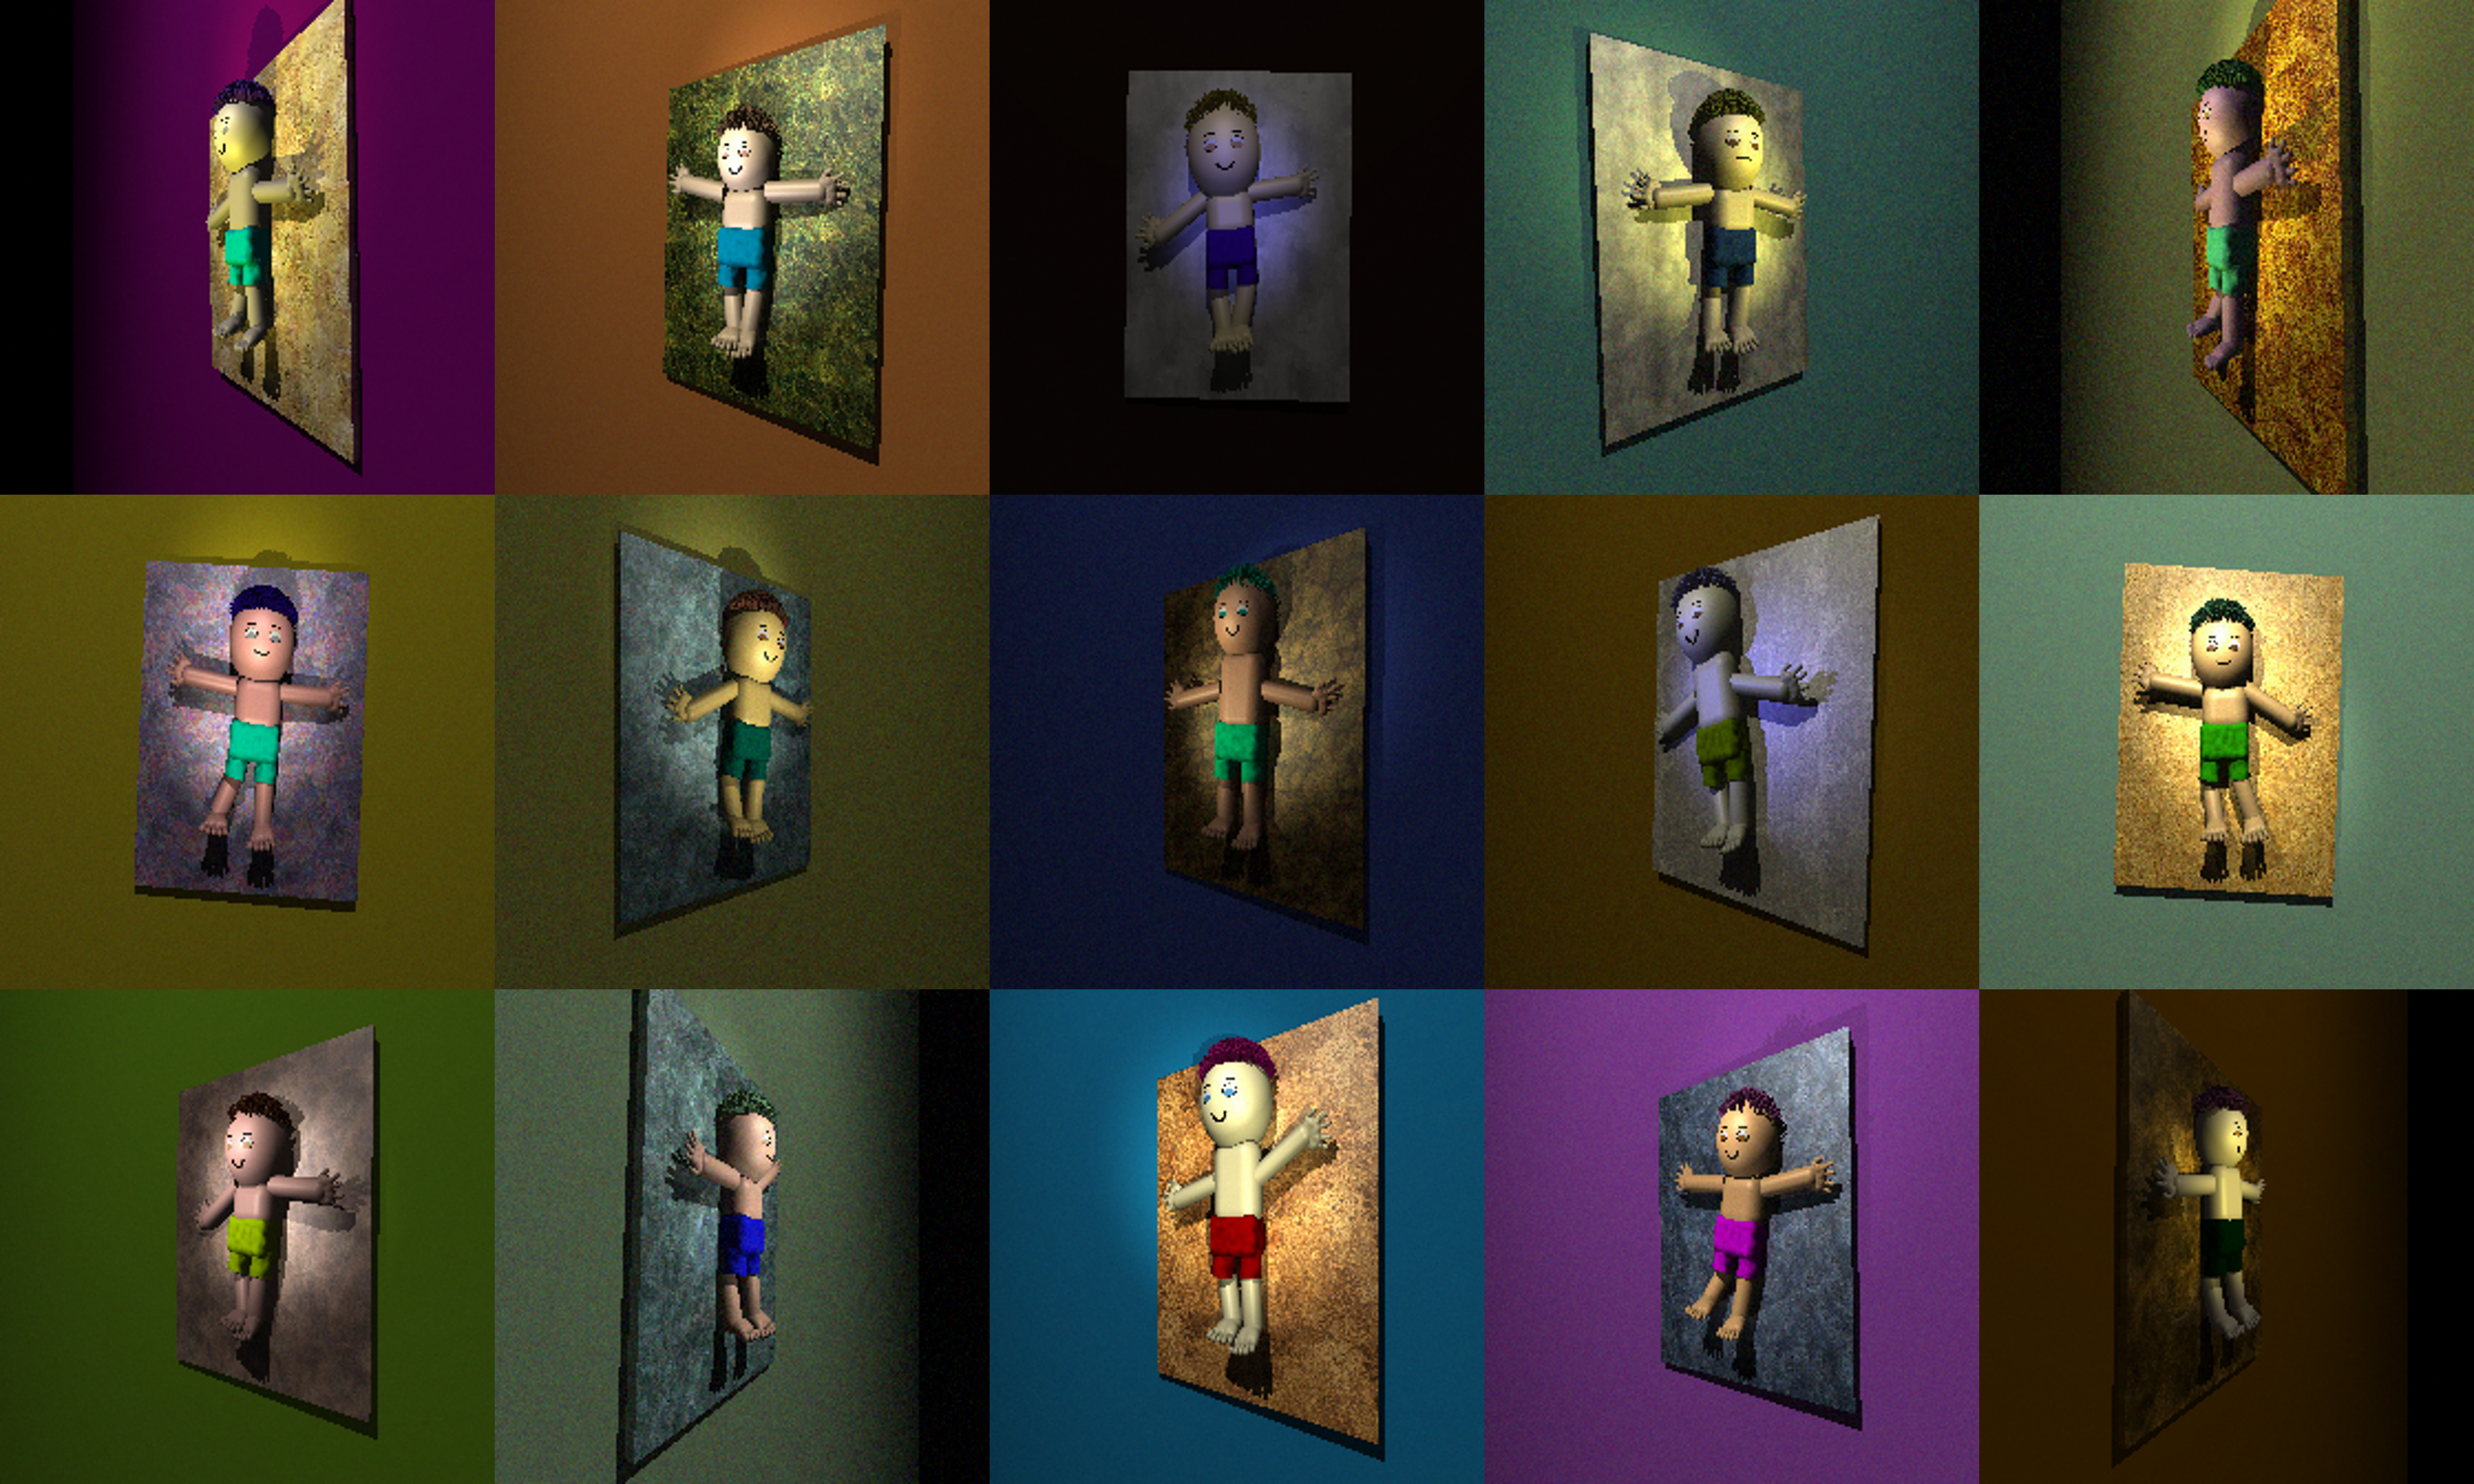
\includegraphics[width=\textwidth]{plots/variety.png}
    \caption{Example of $15$ different synthetic children rendered with default parameters}
    \label{fig:variety}
\end{figure}



\section{Reference}

Tables \ref{table:defaults} and \ref{table:defaults_2} list all the available parameters and their default sample distributions. Table \ref{table:params} provides a listing all standard command line arguments. For example, to set the output resolution to $512 \times 512$ pixels, one would use the following command:

\begin{lstlisting}[language=bash]
python render_children.py --resy 512 --resx 512\end{lstlisting}

Table \ref{table:eye_colors} provides a list of available eye colors.

\begin{table}[h]
    \centering
    {\scriptsize
    \begin{tabular}{|l|l|l|l|}
    \hline
    \textbf{Parameter} & \textbf{Distribution} & \textbf{Parameters} & \textbf{Description} \\ 
    \hline
    \texttt{head\_size} & normal & 0.8, 0.2 & The size of the head\\ 
    \texttt{skin\_color} & color & (1, 0.8, 0.6), (0.1, 0.1, 0.1) & RGB skin color\\ 
    \texttt{shorts\_color} & color & (0.5, 0.5, 0.5), (0.5, 0.5, 0.5) & RGB shorts color \\ 
    \texttt{mat\_texture} & integer & 101, 200 & Mat texture name \\ 
    \texttt{camera\_distance} & normal & 6.2, 0.2 & Distance of camera to child \\ 
    \texttt{rotation\_adj} & normal & 0.0, 4.0 &  Arm rotation adjustment\\ 
    \texttt{right\_arm\_angle\_xy} & normal & 0.0, 10.0 &  Right arm rotation xy\\ 
    \texttt{left\_arm\_angle\_xy} & normal & 0.0, 10.0 &  Left arm rotation xy\\ 
    \texttt{right\_arm\_angle\_z} & normal & 0.0, 5.0 &  Right arm rotation z\\ 
    \texttt{left\_arm\_angle\_z} & normal & 0.0, 5.0 &  Left arm rotation z\\ 
    \texttt{left\_leg\_angle\_xy} & normal & 0.0, 10.0 & Left leg rotation xy  \\ 
    \texttt{right\_leg\_angle\_xy} & normal & 0.0, 10.0 & Right leg rotation xy  \\ 
    \texttt{right\_leg\_angle\_z} & normal & 0.0, 5.0 &  Left leg angle z\\
    \texttt{left\_leg\_angle\_z} & normal & 0.0, 5.0 &  Left leg angle z\\ 
    \texttt{body\_height} & normal & 2.48, 0.16 & Height of main body \\ 
    \texttt{body\_width} & normal & 0.8, 0.1 & Width of the main body \\
    \texttt{body\_depth} & normal & 0.3, 0.1 & Depth of the main body \\
    \texttt{light\_x} & unif & -5.0, 5.0 & X position of primary light  \\ 
    \texttt{light\_y} & unif & -5.0, 5.0 & Y position of primary light \\ 
    \texttt{light\_z} & unif & -5.0, 5.0 & Y position of primary light \\ 
    \texttt{light1} & unif & 0.3, 1.0 & Intensity of light 1 (primary) \\ 
    \texttt{light2} & unif & 0.3, 1.0 & Intensity of light 2 (point light) \\ 
    \texttt{light3} & unif & 0.2, 1.0 & Intensity of light 3 (spotlight 1) \\
    \texttt{light4} & unif & 0.3, 1.0 & Intensity of light 4 (spotlight 2) \\ 
    \texttt{backcolor\_red} & unif & 0.0, 1.0 & Background color red \\ 
    \texttt{backcolor\_green} & unif & 0.0, 1.0 &  Background color green\\ 
    \texttt{backcolor\_blue} & unif & 0.0, 1.0 & Background color blue \\ 
    \texttt{haircolor\_red} & unif & 0.0, 1.0 &  Hair color red\\ 
    \texttt{haircolor\_green} & unif & 0.0, 1.0 & Hair color green \\ 
    \texttt{haircolor\_blue} & unif & 0.0, 1.0 & Hair color blue \\ 
    \texttt{eye\_color\_index} & integer & 0, 9 & Eye color number \\ 
    \texttt{smile\_factor} & unif & -40.0, 100.0 & Smiling factor (100=full smile) \\ 
    \texttt{mat\_rotate\_y} & unif & -2.0, 2.0 & Mat rotation y axis \\ 
    \texttt{mat\_rotate\_z} & unif & -3.0, 3.0 & Mat rotation x axis \\ 
    \texttt{child\_rotate\_y} & normal & 0.0, 6.0 & Child rotation y axis \\ 
    \texttt{child\_rotate\_z} & normal & 0.0, 6.0 & Child rotation z axis \\ 
    \texttt{child\_rotate\_x} & normal & 0.0, 0.01 & Child rotation x axis \\ 
    \texttt{hair\_count} & unif & 250, 4000 & Number of hair follicles \\
    \texttt{hair\_length} & unif & 0.10, 0.18 & Average hair length \\ 
    \texttt{image\_noise\_level} & unif & 0.0, 8.0 & Gaussian image noise level\\ 
    \texttt{image\_box\_level} & unif & 0.0, 0.01 & Box image noise level \\
    \texttt{child\_shift\_x} & unif & -0.05, 0.05 & Child translation x\\
    \texttt{child\_shift\_y} & unif & -0.05, 0.05 & Child translation y\\
    \texttt{child\_shift\_z} & unif & -0.05, 0.05 & Child translation z\\
    \texttt{foot\_size} & unif & 0.15, 0.23 & Foot size\\
    \texttt{hand\_size} & unif & 0.12, 0.21 & Hand size\\
    \texttt{average\_finger\_length} & unif & 0.05, 0.08 & Average finger length\\
    \texttt{average\_toe\_length} & unif & 0.03, 0.05 & Average toe length\\
    \texttt{light\_1\_color\_red} & unif & 0.5, 1.0 & Light 1 color red\\
    \texttt{light\_1\_color\_green} & unif & 0.5, 1.0 & Light 1 color green\\
    \texttt{light\_1\_color\_blue} & unif & 0.5, 1.0 & Light 1 color blue\\
    \texttt{light\_2\_color\_red} & unif & 0.5, 1.0 & Light 2 color red\\
    \texttt{light\_2\_color\_green} & unif & 0.5, 1.0 & Light 2 color green\\
    \texttt{light\_2\_color\_blue} & unif & 0.5, 1.0 & Light 2 color blue\\
    \texttt{light\_3\_color\_red} & unif & 0.5, 1.0 & Light 3 color red\\
    \texttt{light\_3\_color\_green} & unif & 0.5, 1.0 & Light 3 color green\\
    \texttt{light\_3\_color\_blue} & unif & 0.5, 1.0 & Light 3 color blue\\
    \texttt{light\_4\_color\_red} & unif & 0.1, 0.3 & Light 4 color red\\
    \texttt{light\_4\_color\_green} & unif & 0.1, 0.3 & Light 4 color green\\
    \texttt{light\_4\_color\_blue} & unif & 0.1, 0.3 & Light 4 color blue\\
    \texttt{light\_1position\_x} & unif & -5.0, 5.0 & Light 1 position x\\
    \texttt{light\_1position\_y} & unif & -5.0, 5.0 & Light 1 position y\\
    \texttt{light\_1position\_z} & unif & -5.0, 5.0 & Light 1 position z\\
    \texttt{light\_2position\_x} & unif & -5.0, 5.0 & Light 2 position x\\
    \texttt{light\_2position\_y} & unif & -5.0, 5.0 & Light 2 position y\\
    \texttt{light\_2position\_z} & unif & -5.0, 5.0 & Light 2 position z\\
    \hline
    \end{tabular}
    }
    \caption{ChildSynth default parameters part 1}
    \label{table:defaults}
\end{table}

\begin{table}[h]
    \centering
    \scriptsize
    \begin{tabular}{|l|l|l|l|}
    \hline
    \textbf{Parameter} & \textbf{Distribution} & \textbf{Parameters} & \textbf{Description} \\ 
    \hline
    \texttt{matt\_width} & unif & 3.0, 4.0 & The width of the mat\\
    \texttt{matt\_height} & unif & 3.0, 4.0 & The height of the mat\\
    \texttt{matt\_thickness} & unif & 3.0, 4.0 & The mat's average thickness\\
    \texttt{matt\_wrinkle\_height} & normal & 0.1, 0.01 & mat's average wrinkle height\\
    \texttt{matt\_wrinkle\_freq} & normal & 0.4, 0.02 & mat's wrinkle frequency\\
    \texttt{matt\_texture} & choice & 100 & The texture of the mat\\
    \texttt{image\_noise\_level} & unif & 0.0, 8.0 & Gaussian image noise level\\
    \texttt{image\_noise\_box} & constant & 0.0 & Box image noise level\\
    \texttt{eye\_color\_index} & choice & 10 & Eye color index\\
    \texttt{eye\_size} & normal & 0.1, 0.01 & Eye size\\
    \texttt{eyebrow\_height} & normal & 0.1, 0.01 & Eyebrow height\\
    \texttt{eyebrow\_width} & normal & 0.1, 0.01 & Eyebrow width\\
    \texttt{eyebrow\_spacing} & normal & 0.09, 0.005 & Eyebrow spacing\\
    \texttt{mouth\_width} & normal & 0.12, 0.012 & Mouth width\\
    \hline
    \end{tabular}
    \caption{ChildSynth default parameters part 2}
    \label{table:defaults_2}
\end{table}

\begin{table}[h]
    \centering
    \scriptsize
    \begin{tabular}{|l|l|l|}
    \hline
    \textbf{Parameter} & \textbf{Default} & \textbf{Description} \\ 
    \hline
    \texttt{resx} & 512 & The width in pixels of the image\\
    \texttt{resy} & 512 & The height in pixels of the image\\
    \texttt{seed} & not set & An optional random seed for reproducibility\\
    \texttt{num\_children} & 1 & The number of children to render\\
    \hline
    \end{tabular}
    \caption{ChildSynth standard arguments}
    \label{table:params}
\end{table}

\begin{table}[h]
    \centering
    \begin{tabular}{|l|c|}
    \hline
    \textbf{Eye Color} & \textbf{RGB Values} \\
    \hline
    Dark Brown & (0.39, 0.26, 0.13) \\
    \hline
    Light Brown / Hazel & (0.58, 0.34, 0.10) \\
    \hline
    Blue & (0.26, 0.50, 0.72) \\
    \hline
    Green & (0.15, 0.58, 0.40) \\
    \hline
    Amber & (0.77, 0.57, 0.39) \\
    \hline
    Gray & (0.58, 0.58, 0.58) \\
    \hline
    Honey & (0.82, 0.70, 0.55) \\
    \hline
    Teal & (0.0, 0.5, 0.5) \\
    \hline
    Golden & (0.70, 0.42, 0.14) \\
    \hline
    Copper & (0.62, 0.32, 0.17) \\
    \hline
    \end{tabular}
    \caption{Available eye colors and their RGB values}
    \label{table:eye_colors}
\end{table}

\bibliographystyle{unsrt}
\bibliography{references}


\end{document}